% Intended LaTeX compiler: pdflatex
\documentclass[10pt,a4paper,UTF8]{article}
\usepackage{zclorg}
\author{emacsun}
\date{}
\title{spacemacs 快速打开常用文件}
\hypersetup{
 pdfauthor={emacsun},
 pdftitle={spacemacs 快速打开常用文件},
 pdfkeywords={},
 pdfsubject={},
 pdfcreator={Emacs 25.0.50.1 (Org mode 9.0.5)},
 pdflang={English}}
\begin{document}

\maketitle
\tableofcontents
\titlepic{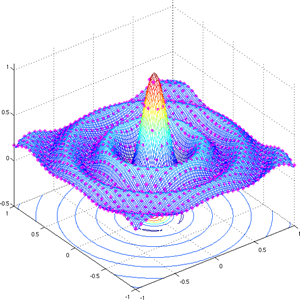
\includegraphics[scale=0.25]{../../img/sinc.PNG}}
使用Emacs久了,总有几个文件是需要经常打开的,比如:emacs的配置文件 \texttt{init.el} 。我使用 \texttt{Org} 维护了一个本地静态博客,这个博客的home文件 \texttt{index.org} 也是我经常访问的文件。时间久了,即使用emacs的 \texttt{bookmark} 功能快速打开,也显得很繁琐无趣。

所幸,spacemacs 已经为 \texttt{init.el} 配置了打开快捷键 \texttt{SPC f e d} 。今天我要为 \texttt{index.org} 绑定一个快捷键。这属于文件类方问快捷键,应该放在 \texttt{SPC f} 为前缀的快捷键下面。使用 \texttt{which-key} 发现 \texttt{SPC f i} 这个组合开没有使用,正好适合用来打开 \texttt{index.org}


\section{快捷键绑定}
\label{sec:org55dce71}


常规的绑定是这样的:
\lstset{language=Lisp,label= ,caption= ,captionpos=b,numbers=none}
\begin{lstlisting}
(global-set-key (kbd "<f6>") (lambda() (interactive)(find-file "~/.emacs")))
\end{lstlisting}
在spacemacs中,快捷键当然要分门别类,方便手指记忆:
\lstset{language=Lisp,label= ,caption= ,captionpos=b,numbers=none}
\begin{lstlisting}
(spacemacs/set-leader-keys "fi" (lambda() (interactive)(find-file "~/.spacemacs.d/init.el")))
\end{lstlisting}

这种方法用 \texttt{SPC f i} 调用一个 \texttt{lambda} 函数。
\section{好用的寄存器}
\label{sec:org371b465}


谷歌告诉我还可以使用寄存器的方法

\lstset{language=Lisp,label= ,caption= ,captionpos=b,numbers=none}
\begin{lstlisting}
(set-register ?e (cons 'file "~/.emacs"))
\end{lstlisting}

使用 \texttt{e} 命名一个寄存器,然后指向文件,使用 \texttt{C-x r j e} 就可以打开了.

目前先使用两种方法,看看哪种效果最好。
\end{document}
